\section{Experimental Design}
To test the hypothesis that the sparsity of the long-range mechanism can lead to a significant processing difficulty at the embedded dependency, we created a two-by-two design that manipulates the above two conditions: (1) whether the two dependencies are \textit{successive} or \textit{nested}, and (2) whether the embedded dependency is \textit{short} or \textit{long} range. Figure \ref{fig:design} describes the resulting four NA-tasks: Short-Successive, Long-Successive, Short-Nested and Long-Nested ('Short' and 'Long' therefore refer to the length of the embedded dependency only).\footnote{\citet{Gulordava:etal:2018} made available several NLMs in several languages, whose hyperparameters were carefully optimized by conducting an extensive grid search. These NLMs were since used in many subsequent studies \citep{}. In our initial work \citep{lakretz2019emergence}, we explored the English NLM made available by this work, howoever, in this current work, since we found that the overall performance of the Italian NLM was better on the more demanding nested construction, we conducted all experimetns with this model, in both NLMs and humans.} 

The successive tasks serve as control tasks, which minimally differ from the nested ones up to the embedded verb, by only a single word ('dice' ('says') in figure \ref{fig:design}). Note also that tasks that have a long embedded dependency have a third noun, which serves as a possible attractor inside the embedded dependency.

For each NA-task, we generated various \textit{conditions} by varying the number of the main and embedded noun, and of the attractor, Short-Successive and Short-Nested have each four conditions corresponding to the possible assignments of numbers to the main and embedded subjects - SS, SP, PS and PP. Similarly, Long-Successive and Long-Nested have eight conditions, based on the possible numbers of the main, embedded subject and attractor - SSS, SSP, SPS, etc. In what follows, by \textit{congruent subjects} we refer to conditions in which the main and embedded subjects share grammatical number (SS, PP, SSS, SSP, PPS and PPP), and by \textit{incongruent subjects} to the rest (SP, PS, SPS, etc.). By \textit{congruent attractor} we refer to conditions in which the embedded subject and the third noun share grammatical number (SSS, SPP, PSS and PPP), and by \textit{incongruent attractor} to conditions in which they differ (SSP, SPS, PSP, PPS) (Methods). 

To anticipate the results, we describe predictions specific for each task, and for each of its verbs, without currently specifying predictions for specific conditions (table \ref{tbl:predictions}). For Short- and Long-Successive, no significant processing difficulties are predicted on the main nor embedded verbs, since the long-range mechanism can in principle encode the grammatical number sequentially: once the long-range agreement mechanism finished processing the first dependency, its grammatical number can be removed from the long-range number units, before encoding the subsequent number of the embedded subject. For Short- and Long-Nested, the long-range mechanism is predicted to successfully process the main dependency and therefore no significant difficulties are predicted on the main verb, beyond the well-known relative difficulty to process center-embeddings, as reported for both humans \citep{traxler2002processing} and NLMs \citep{marvin2018targeted}. In contrast, the embedded dependency in Short-Nested cannot rely on the long-range agreement mechanism, as it is taken up in processing the main one, and therefore the processing of the embedded dependency can only rely on short-range mechanisms, which might not be as robust as the long-range one. To indicate the lack of clear prediction in this case, we mark both options in the table. Finally, in Long-Nested, the performance on the embedded verb is predicted to be significantly low, given that the long-range mechanism can process only a single agreement, as described above. 

\begin{center}
\begin{table}
\centering
\begin{tabular}{|P{3.5cm}||P{3.5cm}|P{3.5cm}|}
    \hline
    \B Sentence Type & \B Main Verb & \B Embedded Verb \\
    \hline
    Successive-Short & V  & V \\
    \hline
    Successive-Long & V & V \\
    \hline
    Nested-Short & V & - \\
    \hline
    Nested-Long & V & X \\
    \hline
\end{tabular}
\caption{A summary of the predictions of model performance on successive and nested dependencies based on the sparsity of the long-range mechanism. 'V' and 'X' represent high and low predicted performance on the agreement task, respectively. Due to possible compensation mechanisms carried by the short-range number units, we make no precise predictions regarding performance on the embedded verb of Nested-Short.}
\label{tbl:predictions}
\end{table}
\end{center}

\begin{figure*}
    \centering
    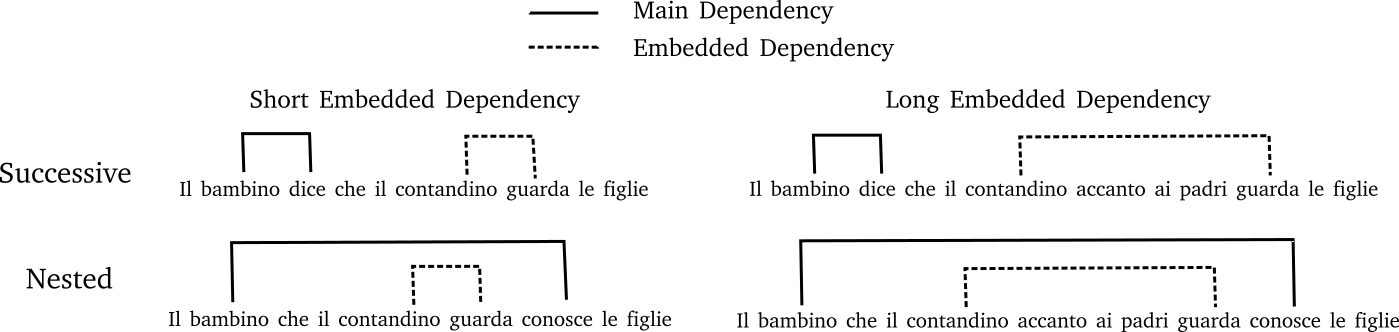
\includegraphics[width=\textwidth]{figures/design.png}
    \caption{\textbf{A full-factorial design for two subject-verb dependencies}. Human subjects and Neural Language Models (NLMs) were presented with sentences from four different syntactic structures, which all have two subject-verb dependencies: a main dependency (continuous lines) and an embedded dependency (dashed). The first factor of the design determines whether the two dependencies are \textit{successive} (top structures) or \textit{nested} (bottom), depending on whether the structure has a sentential complement (SC) or an object-extracted relative clause (objRC), respectively. The second factor determines whether the embedded dependency is \textit{short} (left side) or \textit{long} (right). We refer to the four resulting structures as: SC-short, SC-long, objRC-short and objRC-long.}
    \label{fig:design}
\end{figure*}
